\section{Einführungsphase}
Während der Entwicklung wurde besonderer Wert darauf gelegt, die Anwendung so benutzerfreundlich wie möglich zu gestalten.
Die Einführung der Anwendung beim Kunden wurde in mehreren Schritten durchgeführt, um einen reibungslosen Betrieb zu gewährleisten.

\begin{itemize}
  \item Beantragung und Einrichtung der \acrshort{VM}
  \item Installation der Anwendung auf der \acrshort{VM}
  \item Durchführung eines Tests in \Gls{Checkmk}, um die Funktionsfähigkeit sicherzustellen
\end{itemize}

\noindent
Im Anschluss an das Deployment fand eine Schulung statt, in der dem Kunden die Bedienung der Anwendung nähergebracht wurde.
Dabei wurde gezeigt, wie die Anwendung gestartet und die Verbindung zu \Gls{MetricQ} hergestellt wird.
Ebenso wurde demonstriert, wie Änderungen an der Konfiguration vorgenommen werden können und wie diese Änderungen von der Anwendung erfasst werden.

\noindent
Sobald die Anwendung korrekt funktioniert, wird in der Weboberfläche von \Gls{Checkmk} beispielsweise ein solcher Eintrag angezeigt:

\begin{figure}[H]
  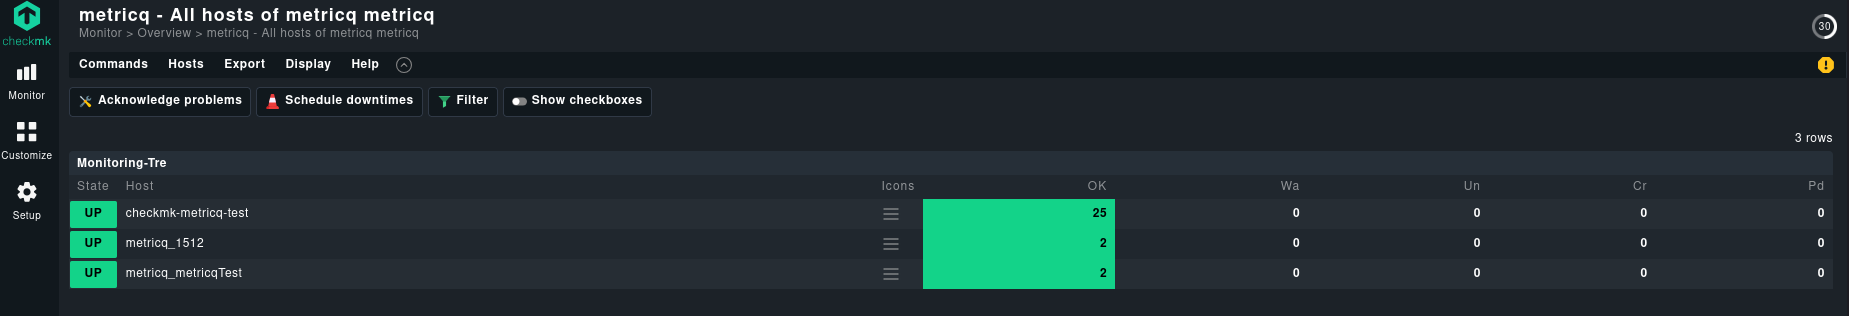
\includegraphics[width=\textwidth]{images/uebersicht_checkmk.png}
  \caption{Übersicht der Anwendung in \Gls{Checkmk}}
  \label{fig:checkmk_uebersicht}
\end{figure}

\noindent
In der Übersicht ist der Agent der Anwendung zu sehen, hier mit dem Namen \textit{checkmk-metricq-test}, sowie die einzelnen Hosts mit den jeweiligen Checks.
Ein Beispiel für den Aufbau der Checks in der Weboberfläche ist ebenfalls in der \reference{fig:checkmk_check_uebersicht} im Anhang zu sehen.
